
%%%%%%%%%%%%%%%%%%%%%%%%%%%%%%%%%%%%%%%%%%%%%%%%%%%%%%%%%%%%%%% 
\section{zkASM Instructions Set} \label{sec:instructions}

\subsection{Memory Related Instructions}


We refer to the memory as a volatile read-write data storage that exists only during the execution of a zkASM program. The memory is divided into different contexts of \texttt{0x40000} words. Each word is 256 bits in length, so each context is \texttt{8MB} in size.

Each context is divided into the following three blocks:

\begin{itemize}
    
\item \textbf{VARS:} With a relative offset of \texttt{0x00000} and a height of \texttt{0x10000} words (\texttt{2MB}), contains the local (and some global ones) context variables pre-defined in the language. The list of all context variables can be found at \href[]{https://github.com/0xPolygonHermez/zkevm-rom/blob/main/main/vars.zkasm}{\texttt{vars.zkasm}}. 

\item \textbf{STACK:} With a relative offset of \texttt{0x10000} and a height of \texttt{0x10000}  words  (\texttt{2MB}), contains the stack of the the EVM. \textbf{STACK} is defined once per context.

\item \textbf{MEMORY:} With a relative offset of \texttt{0x20000} and a height of \texttt{0x20000} words (\texttt{4MB}), contains the free memory that can be freely used. \textbf{MEMORY}, like \textbf{STACK}, is also defined once per context. 
    
\end{itemize}


\begin{figure}[H]
    \centering
    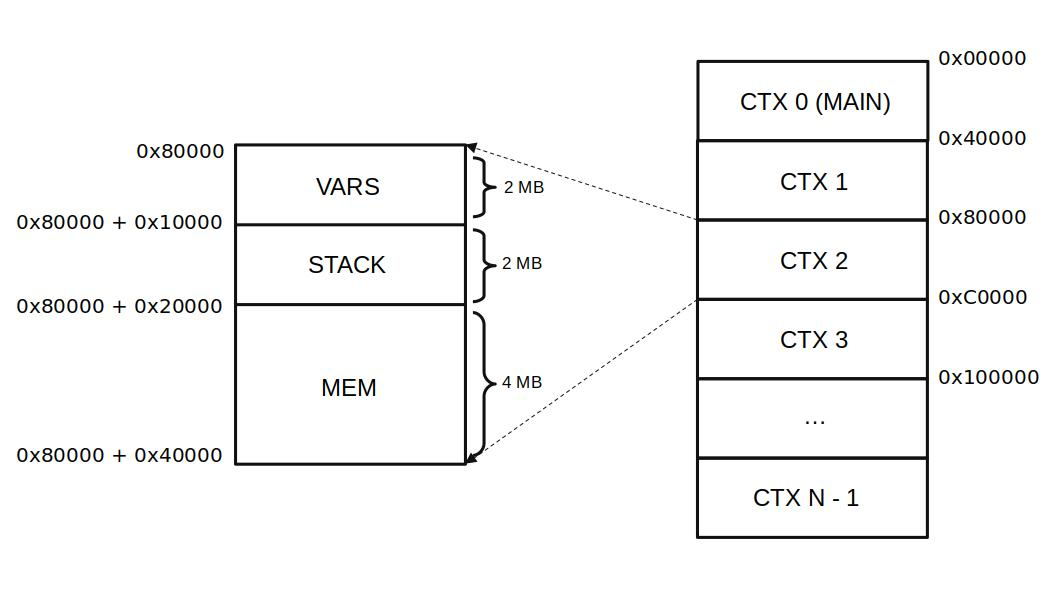
\includegraphics[width=0.6\columnwidth]{\assemblydir/figures/memory-regions}
    \caption{Schema of contexts and memory regions of the zkEVM.}
    \label{fig:memory-regions}
\end{figure}


In order to allow runtime interaction with memory, zkASM has a couple of instructions to read and write values to it. Let us first define how can be access to a specific address of the memory. Memory acess will be parametrized by $2$ integer parameters: the address \addr and the relative address \relAddr. 

\begin{itemize}

\item \addr: Address would be able to define a memory access up to memory region level. That is, \addr will contain information of which context access the memory and if the access is directed to the system variables \textbf{VARS}, the \textbf{STACK} or the \textbf{MEMORY}. Hence, we can compute \addr as follows:

\[
\addr = \texttt{0x40000} \cdot \texttt{CTX} + \texttt{0x10000} \cdot \texttt{isStack} + \texttt{0x20000} \cdot \texttt{isMem}.
\]

being \texttt{isStack} $1$ whenever we are accessing to the \textbf{STACK} memory region and $0$ otherwise and similarly with \texttt{isMem}. Observe that \texttt{isStack} and \texttt{isMem} can not be both equal to $1$ at the same time. Moreover, it is worth noticing that we are pointing to the \textbf{VARS} region whenever \texttt{isStack} and \texttt{isMem} are both $0$.

\item \relAddr: However, \addr is not enough. Hence, \relAddr will point to a specific memory slot inside a concrete memory region of a context. We should take into account that \relAddr can never be negative. Moreover, \relAddr is also bounded from above: if we are accessing to the \textbf{MEMORY}, \relAddr should be strictly less than \texttt{0x40000} (because memory measures $\texttt{4MB}$) and if we are accessing to the \textbf{STACK} or to the system variables \textbf{VARS}, \relAddr should be strictly less than \texttt{0x10000} (because both memory regions measure $\texttt{2MB}$). Then, the wanted memory slot will be equal to $\addr + \relAddr$.

\end{itemize}

Let us know how to specify \addr and \relAddr in zkASM language. We can specify \addr with $3$ keywords: \texttt{SYS} (which corresponds to \textbf{VARS} memory region), \texttt{STACK} (which corresponds to \textbf{STACK} memory region) and \texttt{MEM} (which corresponds to \textbf{MEMORY} memory region). Invoking \texttt{STACK} will increase \addr by $\texttt{0x10000}$ and similarly, invoking \texttt{MEM} will increase \addr by \texttt{0x20000}. However, since \textbf{VARS} is the first memory region, it will not produce an increase in \addr. Moreover, \addr will also increase depending on the current context. More specifically, a total amount of \texttt{0x40000} will be increased per context, following our memory description above. 

To specify \relAddr we can use $2$ registers: \E and \RR. If \E is chosen, \relAddr will increase a total amount of $\E_0$ units. Similarly, if \RR is chosen, \relAddr will increase by \RR. Moreover, we can add a numeric offset to increase a fixed amount of units \addr + \relAddr. 

The syntax will be, in each case:

\begin{zkasm}
addr:relAddr 
; or
addr:relAddr+offset
; or 
addr:relAddr-offset
\end{zkasm}

Moreover, the stack pointer \SP will be also affecting the computation of \SP in the case we are pointing directly to the \textbf{STACK} region. Accessing to the \textbf{STACK} can be do it in two ways: the one explained before by invoking \texttt{STACK} keyword or using the \SP register. The later, and most common one, will be explained later on, in Section \ref{sec:stack}. Hence, \relAddr can be computed as follows:

\[
\relAddr = \texttt{useE} \cdot \E_0 + \texttt{useRR} \cdot \RR + \texttt{isStack} \cdot \SP + \offset.
\]

Below, we specify concrete examples on how to specify addresses:

\begin{zkasm}
SYS:E
SYS:E+1
STACK:RR
MEM:E 
MEM:E-2
MEM:RR+1
\end{zkasm}

To end up, we can also access to addresses by means of global and local variables, defined elsewhere in the assembly code. This variables will have a unique identifier that we will use in order to access to it.


\subsubsection{\MLOAD}


\MLOAD is the zkASM instruction used to read a value from a specific address in memory. It takes the pointer address of the memory slot to be read as a parameter. We can store the value that is read in a register of our choosing by using the free input (\texttt{\$}) assignment. 

Suppose that we want to read the memory value stored in the address \texttt{someAddr} in a certain context. For example, the address \texttt{someAddr} can be defined by the global variable:
\begin{zkasm}
VAR GLOBAL someAddr
\end{zkasm}

The following zkASM code stores the corresponding value into the register \A:
\begin{zkasm}
$ => A          :MLOAD(someAddr)
\end{zkasm}





\subsubsection{\MSTORE}


\MSTORE is the zkASM instruction used to write a value to a specific address in memory. It takes the pointer address of the memory slot to be read as a parameter, the register that contains the value to be writed must be also specified.

The following example shows how to store in the memory the value of the current context. Note that as the \MSTORE parameter, it is specified the variable that contains the pointer to where current context is stored in the memory. The value stored will be taken from \texttt{CTX} register:
\begin{zkasm}
CTX       :MSTORE(currentCTX)      
\end{zkasm}



\subsubsection{Dealing with the STACK} \label{sec:stack}

A stack machine is a machine in which temporary values for computations are moved to and from a push down stack. Operations over the stack are the typical: \texttt{PUSH}, \texttt{POP}, \texttt{DUP}, \texttt{SWAP}, etc. Since the EVM is a stack-based virtual machine, we reserve an address space to create a stack within the memory of the zkEVM. The classical pointer called \texttt{STACK POINTER} (\texttt{SP}) contains the address of the \textbf{next free position on the} \texttt{STACK}. A \texttt{POP} from the \texttt{STACK} can be implemented as:

\begin{zkasm}
SP -1 => SP
$ => A		:MLOAD(SP)
\end{zkasm}

where we decrement \texttt{SP} to reposition it on the last element of the stack and
then we load this element into registry \A. Similarly, a \texttt{PUSH} into the \texttt{STACK} can be implemented as:

\begin{zkasm}
0		:MSTORE (SP++)
\end{zkasm}

which saves a \texttt{0} at the top of the stack and increments \texttt{SP}. An important note about both the stack and the memory is that the stack pointer and the memory are per context.




\subsubsection{\MEMALIGNRD}

Although the memory word in zkASM is 256 bits long, in roder to mimic the regular Ethereum Virtual Machine (EVM) memory behavior, zkASM has a specific instructions for accessing memory at the byte level. The instruction \MEMALIGNRD enables reading 32 bytes starting from an offset of any byte in memory. In this way, two memory registers are read and a the following transformation is applied to virtually obtain a new 32-byte word as a result of the reading.
\begin{align*}
    \texttt{val} &= \Bigr[ \texttt{m}_0 \ll 8 \cdot \texttt{offset} \Bigr] \mathbin\Vert \Bigr[ \texttt{m}_1 \gg 256- 8 \cdot \texttt{offset} \Bigr] 
\end{align*}

Here, the symbol $\mathbin\Vert$ denotes string concatenation. The registers must be set as follows before call the \MEMALIGNRD instruction. We can store the value that is read in a register of our choosing by using the free input (\texttt{\$}) assignment.


\begin{figure}[h!]
    \renewcommand{\figurename}{Table}
    \[
    \begin{array}{|c|c|}
        \hline
        \mathbf{Register} &\mathtt{MEM\_ALIGN\_RD} \ \mathbf{parameters} \\ \hline
        \A & \texttt{Memory Slot of } \mathtt{m_0} \\
        \B & \texttt{Memory Slot of } \mathtt{m_1} \\
        \C & \texttt{offset} \\
        \hline
    \end{array}
    \]
    \caption{\MEMALIGNRD instruction parameters.}
    \label{tab:memory-first-example}
\end{figure}

The following example shows how to read 32 bytes that are stored occupying part of two consecutive zkASM memory words. The read value will be stored in register \A:

\begin{zkasm}
$ => A          :MLOAD(someAddr)
$ => B          :MLOAD(someAddr+1)
16 => C

$ => A          :MEM_ALIGN_RD
\end{zkasm}

Figure ?? shows how the 32-bytes value will be read for the \MEMALIGNRD given example.

\begin{figure}[H]
    \centering
    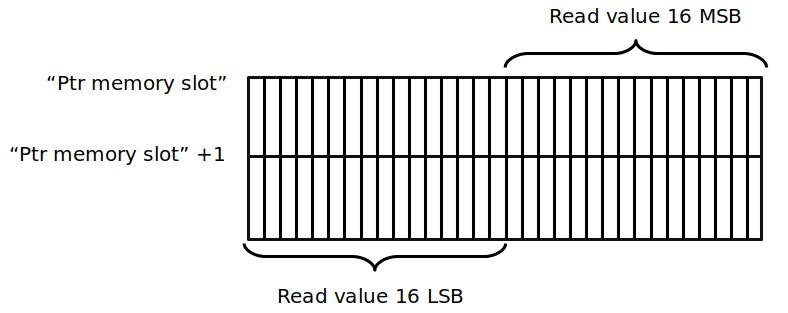
\includegraphics[width=0.8\columnwidth]{\assemblydir/figures/mem-align-wr}
    \caption{Example of how values are read from the memmory using \MEMALIGNRD with an offset of 16.}
    \label{fig:memory-regions}
\end{figure}

\subsubsection{\MEMALIGNWR}
\MEMALIGNWR is equivalent to \MEMALIGNRD but for writing a 32-byte value. In this case, we have to specify two memory slots that will be written after applying the following transformation to the value to be stored. The registers that contains the value to be stored must also be specified.
\begin{align*}
    \texttt{w}_0 &= \Bigr[ \texttt{m}_0 \ \texttt{\&} \ \left(2^{256} - 2^{256-8 \cdot \texttt{offset}} \right) \Bigr] \mathbin\Vert \Bigr[  \texttt{val} \ll 8 \cdot \texttt{offset} \Bigr]  \\
    \texttt{w}_1 &= \Bigr[ \texttt{m}_1 \ \texttt{\&} \ \left( \left( 2^{256} - 1\right)  \gg 8 \cdot \texttt{offset}\right) \Bigr] \mathbin\Vert \Bigr[ \texttt{val} \ll 8 \cdot \texttt{offset} \Bigr] 
\end{align*}

\begin{figure}[h!]
    \renewcommand{\figurename}{Table}
    \[
    \begin{array}{|c|c|}
        \hline
        \mathbf{Register} &\mathtt{MEM\_ALIGN\_WR} \ \mathbf{parameters} \\ \hline
        \A & \texttt{Memory Slot of } \mathtt{m_0}  \\
        \B & \texttt{Memory Slot of } \mathtt{m_1}  \\
        \C & \mathtt{offset} \\
        \D & \mathtt{w_0} \\
        \E & \mathtt{w_1} \\
        \op& \texttt{Value to be written} \\
        \hline
    \end{array}
    \]
    \caption{\MEMALIGNWR instruction parameters.}
    \label{tab:memory-first-example}
\end{figure}

The following example shows how to write 32 bytes that are stored occupying part of two consecutive zkASM memory words. The value to be stored will be taken from free input register:

\begin{zkasm}
$ => A          :MLOAD(MEM:E)
$ => B          :MLOAD(MEM:E+1)

${memAlignWR_W0(A,mem.bytesToStore,C)} => D                    ; no trust calculate W0
${memAlignWR_W1(B,mem.bytesToStore,C)} => E                    ; no trust calculate W1
$               :MEM_ALIGN_WR,MLOAD(bytesToStore)
\end{zkasm}

\subsubsection{\MEMALIGNWRE}

\MEMALIGNWRE allows writing only 8 bits of a specific memory slot. In this case, we have to specify the memory slot to be written, the register that contains the byte to be stored, and the offset value that situates the byte in a specific position of the 32-byte word. The value will be written after applying the following transformation:
\begin{align*}
    \texttt{w}_0 &= \Bigr[ \texttt{m}_0 \ \texttt{\&} \ \left( \texttt{maskByte} \gg 8 \cdot \texttt{offset} \right) \Bigr]  \mathbin\Vert \Bigr[ \left( \texttt{bits} \ \texttt{\&} \ \texttt{0xFF} \right)  \ll 8 \cdot \left( 31-\texttt{offset}\right) \Bigr] 
\end{align*}
where $\texttt{maskByte}$ equals $2^{256} - 1$. 

\begin{figure}[h!]
    \renewcommand{\figurename}{Table}
    \[
    \begin{array}{|c|c|}
        \hline
        \mathbf{Register} &\mathtt{MEM\_ALIGN\_WR8} \ \textbf{parameters} \\ \hline
        \A & \texttt{Memory Slot of } \mathtt{m_0} \\
        \C & \mathtt{offset} \\
        \D & \mathtt{w_0} \\
        \op& \texttt{Value to be written} \\
        \hline
    \end{array}
    \]
    \caption{\MEMALIGNWRE instruction parameters.}
    \label{tab:memory-first-example}
\end{figure}

The following example shows how to write $1$ bytes stored in the byte $4$ of a specific storage slot. The value to be stored will be taken from \B register:

\begin{zkasm}
4 => C
$ => A          :MLOAD(someAddr)
${memAlignWR8_W0(A,B,C)} => D  ; no trust calculate W0
B               :MEM_ALIGN_WR8 ; only use LSB of B, rest of bytes could be non zero
\end{zkasm}

\subsection{Storage Related Instructions}

Polygon zkEVM, like Ethereum L1, has a storage component for storing persistent on-chain data, which includes the balances of all accounts, their nonces, and the state of all deployed smart contracts along with their codes. The data that forms the state is represented as cryptographic trie, but while Ethereum L1 uses a modified Patricia tree with Keccak256 as the hash operation, Polygon zkEVM uses a binary sparse Merkle tree with Poseidon as the hash operation (refer to the technical documents regarding the zkEVM bridge annex A to learn more about sparse Merkle trees).

Poseidon is a hash function that's specifically designed for use in zero-knowledge applications, as it's meant to operate with values of a prime field and it has been proven to be much more performant than Keccak256 in zero-knowledge constructions like those used in Polygon zkEVM. Moreover Poseidon hash has an input named capacity, which can be used as an extra input value.

Barely, the Polygon zkEVM state tree is a key-value structure in which the integrity can be ensured by a 256-bit value known as the state root. Each entry in the tree is a leaf and directly stores a 256-bit value. Additionally, the index position of that leaf in the tree corresponds to the 256-bits of the key. As can be seen in Figure X, since the keys are 256-bits in length, the tree has 32 levels and a total capacity of $2^{256}$ leaves.


\begin{figure}[H]
    \centering
    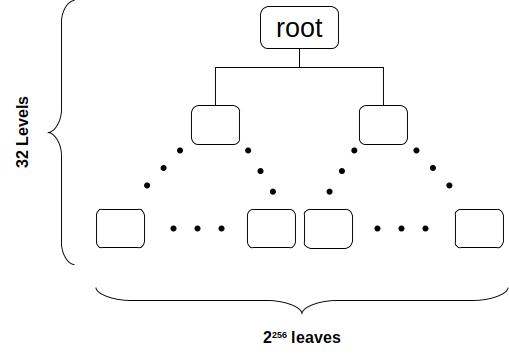
\includegraphics[width=0.6\columnwidth]{\assemblydir/figures/state-trie}
    \caption{Polygon zkEVM state trie.}
    \label{fig:hashk-add-bytes}
\end{figure}

Since five different types of values can be stored, a distinction must be made among the five types of leaves. Table X shows the relation between leaf type and the corresponding data types that they contain.

\begin{figure}[h!]
    \renewcommand{\figurename}{Table}
    \[
    \begin{array}{|c|c|}
        \hline
        \mathbf{Leaf~type} &\mathbf{Data~type} \\ \hline
        \mathtt{0} & \mathtt{Account~balance} \\
        \mathtt{1} & \mathtt{Account~nonce} \\
        \mathtt{2} & \mathtt{Contract~code~hash} \\
        \mathtt{3} & \mathtt{Contract~storage~slot~value} \\
        \mathtt{4} & \mathtt{Contract~code~length} \\
        \hline
    \end{array}
    \]
    \caption{Polygon zkEVM state tree leaf types.}
    \label{tab:memory-first-example}
\end{figure}


For each leaf entered in the tree its key is computed as follows:

$$\texttt{key} = \texttt{Poseidon}(\texttt{key\_seed})$$

where \texttt{key\_seed} is a $32$-bytes integer constructed as follows:
\[
\texttt{key\_seed} = (\texttt{account\_address} \mid\mid \texttt{0x00000000} \mid\mid \texttt{leaf\_type} \mid\mid \texttt{0x00000000})
\]
being $\texttt{account\_address} \in \{0, 1, \dots, 2^{160} - 1\}$ is a $20$-bytes integer and $\texttt{leaf\_type} \in \{0, 1, \dots, 2^{32} - 1\}$ a $4$-bytes integer.

The capacity of the Poseidon's instance used when computing keys is always zero except in the case where the leaf corresponds to a contract storage slot value (leaf type 3), in which case the capacity is directly set to the storage slot pointer. It's important to note that because the contract storage slot pointer is not encoded in the 32-byte input, if we do not use the capacity, all storage slots for the same contract would lead to the same state tree leaf.

Te value sored in the leaf has the following structure:
\[
(v_0, \dots, v_7)
\]
codifying a $256$-bits unsigned integer, where $v_i \in \FF_p$ are bounded to $32$-bits each. 

In order to allow runtime interaction with the Polygon zkEVM state tree zkASM has a couple of instructions to read and write values on it.

\subsubsection{\texttt{SLOAD}}

\texttt{SLOAD} is the zkASM instruction used to read a value from a leaf in the state tree. It takes Poseidon's ``Input" and ``Capacity" parameters, along with the leaf type, to compute the key of the leaf to be read. The registers must be set as follows before call the \texttt{SLOAD} instruction.

\begin{figure}[h!]
    \renewcommand{\figurename}{Table}
    \[
    \begin{array}{|c|c|}
        \hline
        \mathbf{Register} &\texttt{SLOAD } \textbf{parameters} \\ \hline
        \A & \mathtt{Account~address} \\
        \B & \mathtt{Leaf~type} \\
        \C & \mathtt{Contract~storage~slot~pointer~(capacity)} \\
        \hline
    \end{array}
    \]
    \caption{\texttt{SLOAD} instruction parameters.}
    \label{tab:memory-first-example}
\end{figure}

We can store the value that is read in a register of our choosing by using the free input (\texttt{\$}) assignment.

The following example shows how to read the balance of a specific account, the value that is read will be stored in the \E register:

\begin{zkasm}
someAccountAddr => A          
0 => B      
0 => C          
$ => E          :SLOAD
\end{zkasm}

The following example shows how to read a storage slot of a specific contract, the value that is read will be stored in the \E register:

\begin{zkasm}
someAccountAddr => A          
3 => B      
storageSlotPtr => C 
$ => E          :SLOAD
\end{zkasm}

\subsubsection{\texttt{SSTORE}}

\texttt{SSTORE} is the zkASM instruction used to store a value to a leaf in the state tree. It takes Poseidon's ``Input" and ``Capacity" parameters, along with the leaf type, to compute the key of the leaf to be writen, in addition takes the value to be written. The registers must be set as follows before call the \texttt{SSTORE} instruction.

\begin{figure}[h!]
    \renewcommand{\figurename}{Table}
    \[
    \begin{array}{|c|c|}
        \hline
        \mathbf{Register} &\texttt{SSTORE } \textbf{parameters} \\ \hline
        \A & \mathtt{Account~address} \\
        \B & \mathtt{Leaf~type} \\
        \C & \mathtt{Contract~storage~slot~pointer~(capacity)} \\
        \D & \mathtt{Value~to~write} \\
        \hline
    \end{array}
    \]
    \caption{\texttt{SSTORE} instruction parameters.}
    \label{tab:memory-first-example}
\end{figure}

The following example shows how to write a storage slot of a specific contract:

\begin{zkasm}
someAccountAddr => A          
3 => B      
storageSlotPtr => C          
value => D         
A               :SSTORE
\end{zkasm}




%%%%%%%%%%%%%%%%%%%%%%%%%%%%%%%%%%%%%%%%%%%%%%%%%%%%%%%%%%%%%%%

\subsection{Binary-Related Instructions}

The arithmetic operators are used to perform arithmetic mathematical operations on numeric data stored in registers.

\subsubsection{\ADD}

\ADD is used to sum the content of the registers \A and \B, the result will be treated as a free input. The following example shows how to use \ADD instruction.

\begin{zkasm}
val1 => A          
val2 => B          

$ => C             :ADD ; [ val1 + val2 => C]
\end{zkasm}

\subsubsection{\SUB}

\SUB is used to subtract de content fo register \B to \A, the result will be treated as a free input. The following example shows how to use \SUB instruction.

\begin{zkasm}
val1 => A          
val2 => B          

$ => C             :SUB ; [ val1 - val2 => C]
\end{zkasm}



\subsubsection{\LT}

\LT instruction is used to compare the values of the registers \A and \B as \textbf{unsigned integers}. The output of the operation will be $1$ if \A is actually lower than \B (that is, $\A < \B$) and $0$ otherwise (that is, $\A \geq \B$). The output of the instruction will be treated as a free input. The next lines of code show an example on how to use \LT instruction:

\begin{zkasm}
valA => A
valB => B

$ => C			:LT ; [1 if A < B, 0 if A <= B]
\end{zkasm}





\subsubsection{\SLT}

\SLT instruction is used to compare the values of the registers \A and \B as \textbf{signed integers}, explained in Section \ref{sec:binary-sm}. The output of the operation will be $1$ if \A is actually lower than \B (that is, $\A < \B$) and $0$ otherwise (that is, $\A \geq \B$). The output of the instruction will be treated as a free input. The next lines of code show an example on how to use \SLT instruction:

\begin{zkasm}
valA => A
valB => B

$ => C			:SLT ; [1 if A < B, 0 if A <= B]
\end{zkasm}


\subsubsection{\EQ}

\EQ instruction is used to compare the equality relationship between the values of the registers \A and \B. The output of the operation will be $1$ if \A is equal to \B (that is, $\A = \B$) and $0$ otherwise (that is, $\A \neq \B$). The output of the instruction will be treated as a free input. The next lines of code show an example on how to use \EQ instruction:

\begin{zkasm}
valA => A
valB => B

$ => C			:EQ ; [1 if A = B, 0 if A != B]
\end{zkasm}


\subsubsection{\AND}


\AND instruction is used to perform the bit-wise \AND operation between registers \A and \B, as explained in Section \ref{sec:binary-sm}. The output of the instruction will be treated as a free input. The next lines of code show an example on how to use \AND instruction:

\begin{zkasm}
valA => A
valB => B

$ => C			:AND
\end{zkasm}

For sake of completeness, let us propose a more concrete example, where we assign the value $\texttt{0xDBn}$ to \A and the value $\texttt{0x86n}$ to \B. The result of the bit-wise \AND operation is going to be \texttt{0x82n} because
\[
\A = \texttt{0b11011011}, \quad \B = \texttt{0b10000110} \Longrightarrow \C = \texttt{0b10000010}.
\]

\begin{zkasm}
0xDBn => A
0x86n => B

$ => C			:AND ; C = 0x82n
\end{zkasm}

\subsubsection{\OR}

\OR instruction is used to perform the bit-wise \OR operation between registers \A and \B, as explained in Section \ref{sec:binary-sm}. The output of the instruction will be treated as a free input. The next lines of code show an example on how to use \OR instruction:

\begin{zkasm}
valA => A
valB => B

$ => C			:OR
\end{zkasm}

For sake of completeness, let us propose a more concrete example, where we assign the value $\texttt{0xDBn}$ to \A and the value $\texttt{0x86n}$ to \B. The result of the bit-wise \OR operation is going to be \texttt{0xDFn} because
\[
\A = \texttt{0b11011011}, \quad \B = \texttt{0b10000110} \Longrightarrow \C = \texttt{0b11011111}.
\]

\begin{zkasm}
0xDBn => A
0x86n => B

$ => C			:OR ; C = 0xDFn
\end{zkasm}



\subsubsection{\XOR}

\XOR instruction is used to perform the bit-wise \XOR operation between registers \A and \B, as explained in Section \ref{sec:binary-sm}. The output of the instruction will be treated as a free input. The next lines of code show an example on how to use \XOR instruction:

\begin{zkasm}
valA => A
valB => B

$ => C			:XOR
\end{zkasm}

For sake of completeness, let us propose a more concrete example, where we assign the value $\texttt{0xDBn}$ to \A and the value $\texttt{0x86n}$ to \B. The result of the bit-wise \XOR operation is going to be \texttt{0x5Dn} because
\[
\A = \texttt{0b11011011}, \quad \B = \texttt{0b10000110} \Longrightarrow \C = \texttt{0b01011101}.
\]

\begin{zkasm}
0xDBn => A
0x86n => B

$ => C			:XOR ; C = 0x5Dn
\end{zkasm}





%%%%%%%%%%%%%%%%%%%%%%%%%%%%%%%%%%%%%%%%%%%%%%%%%%%%%%%%%%%%%%%
\subsection{Arithmetic-Related Instructions}

\subsubsection{\ARITH}

The \ARITH instruction allows to check field operations. More specifically, it checks a combination of an addition and a product, as explained in Section \ref{sec:arith-sm}. Before calling the \ARITH instruction, registers \A, \B, and \C must be set. The equation that follows will be evaluated using the values of these $3$ registers. It is necessary to specify where the result of the evaluation will be stored. If the evaluation results in an overflow of the output register, the overflow value will be stored in register \D. More specifically, the equation that checks the \ARITH instruction is the following one:

\[
\D \cdot 2^{256} + \op = \A \cdot \B + \C
\]

The following example shows how to use \ARITH instruction. The result of the evaluation will be stored in register \A, and if there is an overflow, it will be stored in register \D:
\begin{zkasm}
valA => A          
valB => B          
valC => C
A            :ARITH ; [ valA * valB + valC => [D,A]]
\end{zkasm}





\subsubsection{\ARITHADDDIFF}

The \ARITHADDDIFF instruction allows to perform additions $P + Q$ over the elliptic curve defined in Section \ref{sec:arith-sm}. This instruction can not perform doublings, since the input points to be added are supposed to be different. This is not explicitly check, but since the doubling formula differs a lot from the distinct point addition formula, the result will be wrong if $P = Q$. The input parameters of the instruction are specified in the table below:

\begin{figure}[h!]
    \renewcommand{\figurename}{Table}
    \[
    \begin{array}{|c|c|}
        \hline
        \mathbf{Register} &\texttt{ARITH\_ECADD\_DIFFERENT } \textbf{parameters} \\ \hline
        \A & x_1, \mathtt{~x~coordinate~of~}P \\
        \B & y_1, \mathtt{~y~coordinate~of~}P \\
        \C & x_2, \mathtt{~x~coordinate~of~}Q \\
        \D & y_2, \mathtt{~y~coordinate~of~}Q \\
        \E & x_3, \mathtt{~x~coordinate~of~}P+Q \\
        \op & y_3, \mathtt{~y~coordinate~of~}P+Q \\
        \hline
    \end{array}
    \]
    \caption{\ARITHADDDIFF instruction parameters.}
    \label{tab:memory-first-example}
\end{figure}

An example on how to use the \ARITHADDDIFF instruction can be seen in the code blow. Observe that we make use of the executor implemented functions \texttt{xAddPointEc(A,B,C,D)} and \texttt{yAddPointEc(A,B,C,D)} which compute the $x$ and the $y$ coordinate of $P + Q$ being $P = (A, B)$ and $Q = (C, D)$ whenever $P \neq Q$. After this is computed, the $x$ coordinate of $P + Q$ is is stored into the memory slot given by the address \texttt{addX} and, similarly, the $y$ coordinate of $P + Q$ is pushed into the memory slot given by the address \texttt{addY}. If we have used incorrect values for the coordinates of $P + Q$, an executor error will pop. This will also be captured when the proof of the batch is generated, since the instruction invocation fills the polynomials of the Arithmetic State Machine correctly. 

\begin{zkasm}
$ => A  						:MLOAD(Px)
$ => B  						:MLOAD(Py)
$ => C  						:MLOAD(Qx)
$ => D  						:MLOAD(Qy)
${xAddPointEc(A,B,C,D)} => E  	:MSTORE(addX)
${yAddPointEc(A,B,C,D)} 		:ARITH_ECADD_DIFFERENT, MSTORE(addY)
\end{zkasm}


\subsubsection{\ARITHADDSAME}

The \ARITHADDSAME instruction allows to perform point doublings $2P$ over the elliptic curve defined in Section \ref{sec:arith-sm}. The input parameters of the instruction are specified in the table below:

\begin{figure}[h!]
    \renewcommand{\figurename}{Table}
    \[
    \begin{array}{|c|c|}
        \hline
        \mathbf{Register} &\texttt{ARITH\_ECADD\_DIFFERENT } \textbf{parameters} \\ \hline
        \A & x_1, \mathtt{~x~coordinate~of~}P \\
        \B & y_1, \mathtt{~y~coordinate~of~}P \\
        \E & x_3, \mathtt{~x~coordinate~of~}2P \\
        \op & y_3, \mathtt{~y~coordinate~of~}2P \\
        \hline
    \end{array}
    \]
    \caption{\ARITHADDDIFF instruction parameters.}
    \label{tab:memory-first-example}
\end{figure}

An example on how to use the \ARITHADDSAME instruction can be seen in the code blow. Observe that we make use of the executor implemented functions \texttt{xDblPointEc(A,B)} and \texttt{yDblPointEc(A,B)} which compute the $x$ and the $y$ coordinate of $2P$ being $P = (A, B)$. After this is computed, the $x$ coordinate of $2P$ is is stored into the memory slot given by the address \texttt{doublePx} and, similarly, the $y$ coordinate of $2P$ is pushed into the memory slot given by the address \texttt{doublePy}. If we have used incorrect values for the coordinates of $2P$, an executor error will pop. This will also be captured when the proof of the batch is generated, since the instruction invocation fills the polynomials of the Arithmetic State Machine correctly. 

\begin{zkasm}
$ => A  					:MLOAD(Px)
$ => B  					:MLOAD(Py)

${xDblPointEc(A,B)} => E  	:MSTORE(doublePx)
${yDblPointEc(A,B)} 		:ARITH_ECADD_SAME, MSTORE(doublePy)
\end{zkasm}









%%%%%%%%%%%%%%%%%%%%%%%%%%%%%%%%%%%%%%%%%%%%%%%%%%%%%%%%%%%%%%%
\subsection{Execution Control Flow Related Instructions}

In order to allow to conditional branch execution of the zkASM programs, 4 different instruction has been included in zkASM instructios set.

\subsubsection{\JMP} % Jump
\JMP is an unconditional jump instruction that always causes a jump in the program's execution flow, regardless of any conditions. It takes an address of the ROM as a parameter to continue the execution flow. To avoid using numeric pointers for jumps, zkASM allows jump destinations to be aliased with custom names. The compiler resolves these aliases and substitutes them with pointers later on.

The following code shows the general usage of \JMP instruction:

\begin{zkasm}
    
; ...
; Executed Code
; ...

        :JMP(destinationLabel)

; ... 
; Non Executed Code
; ... 

destinationLabel:

; ...
; Executed Code
; ...
    
\end{zkasm}

Moreover, we can also parametrize the destination of a jump-like instruction using either the first limb of the register $\E_0$ or the register \RR, using the syntax below:

\begin{zkasm}
        :JMP(RR)
        :JMP(E)
\end{zkasm}

For example, the code below will produce a jump of $5$ units in the execution flow:

\begin{zkasm}
5 => E
            :JMP(E)          
\end{zkasm}

The former syntax will be also available for all the other kind of jumps specified in below sections, including the ones having an else clause.

\subsubsection{\JMPN} % Jump if Negative

\JMPN is a conditional jump instruction that causes a jump in the program's execution flow if a specified register contains a negative number. It takes the address of the ROM as a parameter to continue the execution flow. The register that contains the value to be evaluated must also be specified.

In the following example, the execution flow will be redirected to \texttt{stackUnderflow} in the case that the evaluation of $\SP - 2$ leads to a negative number.

\begin{zkasm}
; check stack underflow
SP - 2          :JMPN(stackUnderflow)
\end{zkasm}

Conditional jumps can also receive an else-clause label. The synatx is very similar:

\begin{zkasm}
A					:JMPN(ifClauseLabel, elseClauseLabel)


ifClauseLabel:
        ; do something
        
        
elseClauseLabel:
        ; do something different
\end{zkasm}

If the value stored in the \A register is negative, then the execution of the program will continue under the \texttt{ifClauseLabel} label. However, if the value of \A is bigger or equal than $0$, then the execution will continue from the label \texttt{elseClauseLabel}. 




\subsubsection{\JMPC} % Conditional jump, if a condition is fullfiled

\JMPC is a conditional jump instruction that causes a jump in the program's execution flow if a specified condition is evaluated  as true. It is used along with the following comparative instructions.
\begin{itemize}
    \item \EQ: Evaluates if register \A value is equal to register \B value.
    \item \LT: Evaluates if register \A value is less than register \B value.
    \item \SLT: Evaluates if register \A value is less than register \B value also comparing negative values.
\end{itemize}

In the following example, the execution flow will be redirected to \texttt{absIsNeg} in the case that the value contained in register \A (namely \val) is a negative number.

\begin{zkasm}
val => A
0 => B
$          :SLT, JMPC(absIsNeg)
\end{zkasm}





\subsubsection{\JMPZ} % Jump if Zero

\JMPZ is a conditional jump instruction that causes a jump in the program's exectuion flow if a specified register contains a 0. In the following example, the execution flow will be redirected to \texttt{readCode} in the case that the value contained in register \A (namely \val) is $0$.

\begin{zkasm}
val => A
A                   :JMPZ(readCode)
\end{zkasm}






\subsubsection{\JMPNC and \JMPNZ}

In addition to all the previously defined execution jumps, there are two more jumps: \JMPNC and \JMPNZ. This kind of jumps works the other way around \JMPC and \JMPZ does. More concretely, in the code below, the execution will jump to the label \texttt{someLabel} if and only if the value stored in the register \A \textbf{is not} zero. Otherwise, if the condition is satisfied, the execution will proceed normally.
\begin{zkasm}

A			:JMPNZ(someLabel)


someLabel:
    ; do something
\end{zkasm}

Hence, the first argument appearing in the instruction denotes now the else-clause. In fact, we can also adopt an if-else structure in this kind of negated instructions:

\begin{zkasm}

A			:JMPNZ(elseLabel, ifLabel)

elseLabel:
    ; do something
    
ifLabel:
    ; do something
\end{zkasm}

In the above piece of code, if the value of \A is not zero, then the execution will jump to the label \texttt{elseLabel} and, otherwise, it will jump to \texttt{ifLabel}. 



\subsubsection{\ASSERT}
\ASSERT is used to ensure that a given register has the same value as register \A. A failing assertion, meaning that the values are unequal, will stop execution and throw error during runtime. Additionally, an execution that contains a failing assertion cannot generate a valid CI proof.

The following code will compare $\val_1$ with $\val_2$, and if they are not equal the execution will be immediately stopped:

\begin{zkasm}
val1 => A
val2 => B
B    		:ASSERT
\end{zkasm}


\subsubsection{Subroutines (\CALL and \RETURN)}


Subroutines allow breaking down the code into smaller sections that can be called by using only a \CALL instruction. A subroutine is designed to be reusable and can be called by other parts of the program. The code of a subroutine always ends with a \RETURN instruction. When a subroutine is called, control is transferred from the main program to the subroutine. The subroutine then executes its code and, when it's finished, control is returned to the point in the main program immediately following the point where the subroutine was called.

An example of subroutine can be the \texttt{ecrecover\_tx} subrutine used in the zkEVM ROM, it is used to recover the signer of a specific ethereum transaction. zkASM code of \texttt{ecrecover\_tx } subrutine can be found \href[]{https://github.com/0xPolygonHermez/zkevm-rom/blob/b27579b89a95a344d09656490a50df5fc67c8417/main/ecrecover/ecrecover.zkasm}{here}.

The following zkASM code shows how to use the \texttt{ecrecover\_tx} subroutine. Once the subroutine is executed, the code will continue on the following line and the recovered address will be in register \A:
\begin{zkasm}
0xd9eba16ed0ecae432b71fe008c98cc872bb4cc214d3220a36f365326cf807d68n => A ; Tx hash
0xddd0a7290af9526056b4e35a077b9a11b513aa0028ec6c9880948544508f3c63n => B ; r
0x265e99e47ad31bb2cab9646c504576b3abc6939a1710afc08cbf3034d73214b8n => C ; s
0x1cn => D ; v
                        :CALL(ecrecover_tx)
\end{zkasm}




\subsubsection{References}

The jump-like instructions we presented earlier provide programmers with the ability to modify the execution flow by jumping to various parts of the code. Similarly, subroutines enable the invocation of other code segments located in different files, allowing for a return to the point of invocation to continue with the original flow. However, what if a programmer wants to jump to a label in a different \texttt{.zkasm} file without returning to the original code? This is where \textbf{References} come in handy.

\textbf{References} allow programmers to combine jump-like instructions with subroutines, which in turn allows for the jumping to a label in another \texttt{.zkasm} file without the need to return to the original code. This results in greater flexibility and modularity in code organization and execution.

To use references, the syntax is as follows:

\begin{zkasm}
:JMP(@someLabel + RR)
\end{zkasm}

Here, \texttt{someLabel} refers to a label located in another \texttt{.zkasm} file. The instruction above jumps to the line of code that corresponds to the value stored in the register \RR under the \texttt{someLabel} label. Additionally, it is possible to parameterize the specific line of code to jump to by adding the value of the first limb of the register $\E_0$ to the reference, as shown below:

\begin{zkasm}
    :JMP(@someLabel + E)
\end{zkasm}

References can also be used for other types of jumps, including conditional jumps with an else condition. For example:

\begin{zkasm}
    :JMPN(@someLabel + RR)
    :JMPZ(@someLabel + E)
    :JMPC(@someLabel + RR, elseLabel)
    ; ...
\end{zkasm}

Moreover, \textbf{References} are also useful even if the tag we are pointing is actually inside the same \texttt{.zkasm} file. This is because, as we have seen before, we can parametrize how many lines we ought to jump \textbf{after} some label using the registers \E and \RR, which we can not using only tag identifiers. 

\subsubsection{\REPEAT}

Although jumps are enough in order to build program loops, a \REPEAT instruction has been introduced in order to easily repeat a certain line of code. The \REPEAT instruction makes use of the \RCX register in order to parametrize the number of times the code should be repeated. To illustrate how to use the \REPEAT instruction, we are going to propose an example:

\begin{zkasm}
10 => A
14 => RCX
A + 2 => A  :REPEAT(RCX)

40  		:ASSERT 
\end{zkasm}

The previous code assigns $10$ to the \A register and $14$ to the repeat counter \RCX. After that, invokes an addition by two units of the \A register, together with the \REPEAT instruction with parameter \RCX. This will make the line of code 

\begin{zkasm}
A + 2 => A
\end{zkasm}

to repeat a total amount of $15$ times, the first one written explicitly in the code and the other $14$ times produced by the \REPEAT instruction. This is something the user should take into account. After that, the \A register will contain the value
\[
10 + 15 \cdot 2 = 40.
\]
Hence, an \ASSERT can be invoked against the value $40$, since \A should be $\op = 40$.  




%%%%%%%%%%%%%%%%%%%%%%%%%%%%%%%%%%%%%%%%%%%%%%%%%%%%%%%%%%%%%%%
\subsection{Hash Related Instructions}

Both implementations in the zkEVM of each of the hashes is exactly the same, henceforth what we explain in this section for the \texttt{KECCAK-256} hash can be applied also for the \texttt{Poseidon} hash. There are $4$ instructions referent to \texttt{KECCAK-256} hashes in the zkEVM assembly language: \HASHK, \HASHKONE, \HASHKLEN and \HASHKDIGEST. Each of them has a different purpose:

\begin{itemize}
    
    \item \HASHK: This instruction is in charge of consecutively keep introducing bytes into the input of the hash. Via this instruction we can introduce a maximum amount of $32$ bytes at the same time. 
    
    \item \HASHKONE: This instruction is does actually the same that the previous instruction but only can introduce $1$ byte at the time. 
    
    \item \HASHKLEN: This instruction is the one that actually performs the hash but actually do not retrieve its digest. 
    
    \item \HASHKDIGEST: This instruction retrieves the previous hash digest performed using the \HASHKLEN instruction. 
    
\end{itemize}

Similarly, there are $4$ instructions referent to \texttt{Poseidon} hashes in the zkEVM assembly language: \HASHP, \HASHPONE, \HASHPLEN and \HASHPDIGEST. Each of them mirrors the same instruction explained in the \texttt{KECCAK-256} case. 



\subsubsection{\HASHK}

Since hash functions can hash an arbitrarily large amount of data but our registers are limited to $32$ bytes, we need a procedure to sequentially keep introducing bytes in order to be hashed together. This is what this instruction is providing: it allows to append from $1$ to $32$ bytes to the current input of the hash. The following registers will be relevant in this instruction: $\mathtt{D_0}$ and \texttt{HASHPOS}. The former will contain the desired bytes we want to append and the later will contain the index of the next position of the bytes array of the input of the hash that we will start to fill. That is, this register will contain the total input bytes that we have previously introduced up to this precise moment. 

\begin{figure}[H]
    \centering
    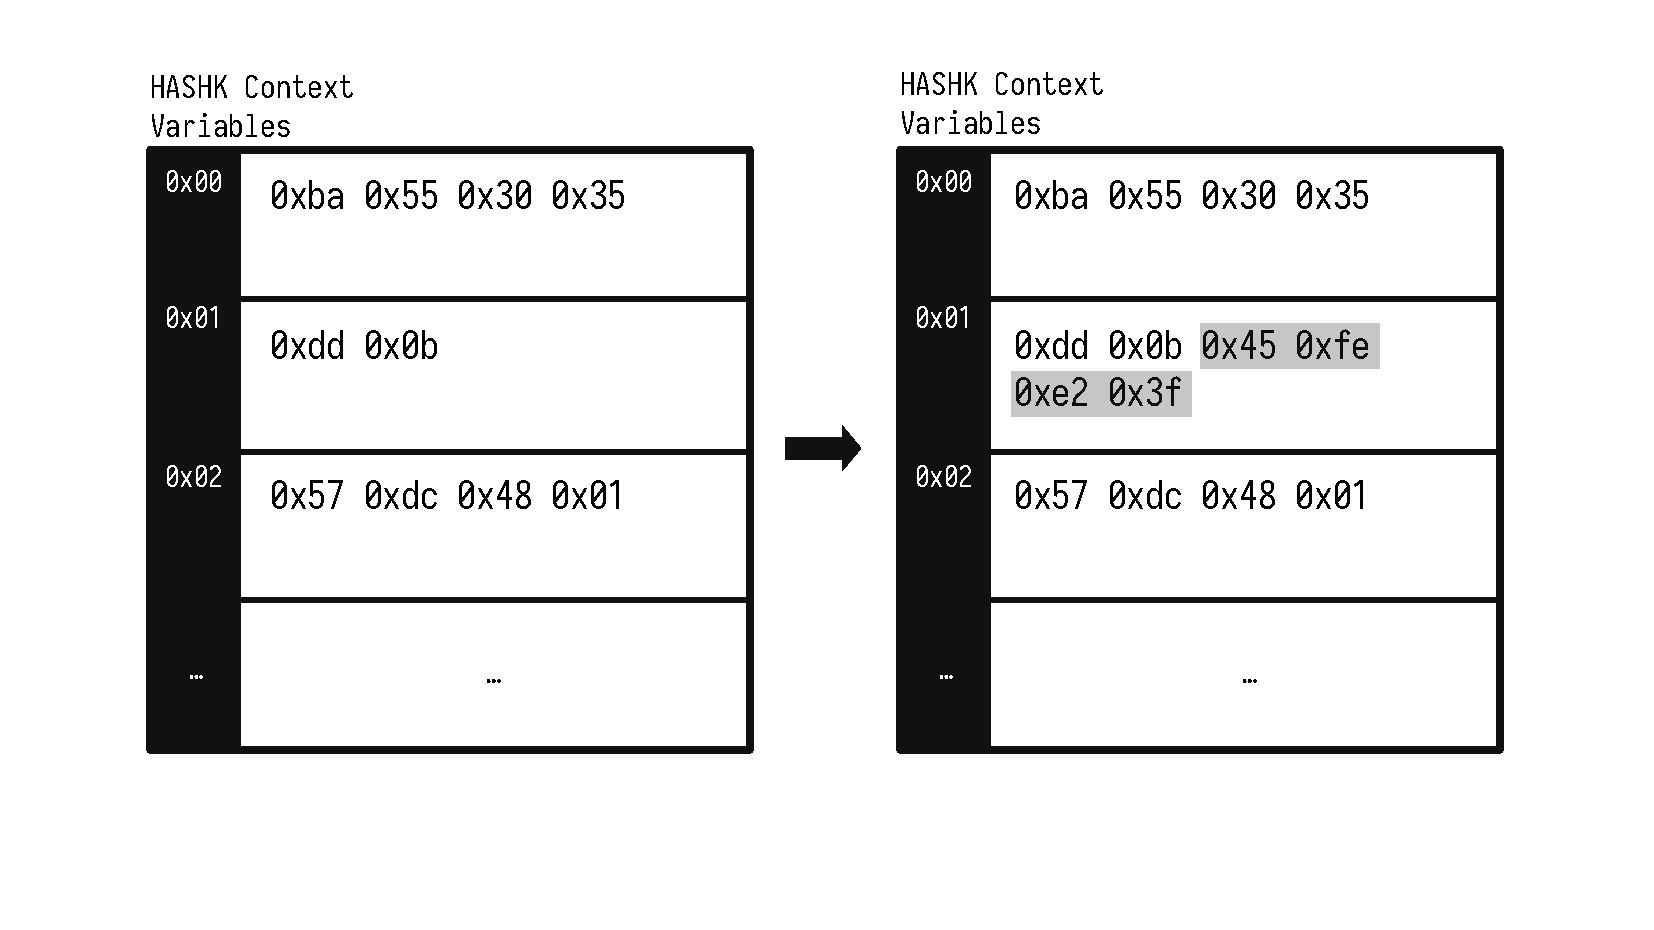
\includegraphics[width=0.6\columnwidth]{\assemblydir/figures/hashk-add-bytes}
    \caption{Schema of the \HASHK instruction.}
    \label{fig:hashk-add-bytes}
\end{figure}

The typical use of the \HASHK instruction in the zkASM language is the following one:

\begin{zkasm}
    op	:HASHK(addr)
\end{zkasm}

The \op placeholder will usually be a register or a register operation like the following one: 

\begin{zkasm}
    A + 1	:HASHK(addr)
\end{zkasm}

We can perform several hashes at the same time, each of them being stored in its corresponding address. Then, we can keep filling each of the addresses' bytes without perturbing the other ones. We can specify the address using the register \E, which is the one used to store addresses $256$-bits, or using a hard coded number. The value $0$ is usually used as an address, which is reserved for storing specific hashes. %TODO: what hashes?

\begin{zkasm}
    A + 1	:HASHK(E)
\end{zkasm}

The former instruction will append the bytes of the current value of \A + 1 into the input of the hash function we want to perform within the bytes attached to the address \E. 

To formalise what the \HASHK instruction does, let $(\op_0, \op_1, \dots, \op_{31})$ be the byte decomposition of the \op variable. We will denote $\mathtt{trunc_{D_0}}(\op)$ by the byte decomposition of \op truncated at the $\mathtt{D_0}$ position. More precisely, 
\[
\mathtt{trunc_{D_0}(\op)} = (\op_0, \op_1, \dots, \op_{\D_0-1}).
\]

Let $\mathtt{hashk}[\texttt{addr}] = (h_0, \dots, h_{\texttt{HASHPOS}})$ be the current array of bytes that we are willing to hash at a certain address \texttt{addr}. The \HASHK instruction will append the $\mathtt{trunc_{D_0}}(\op)$ array into the $\mathtt{hashk}$ one, so that the next state of the (temporal) input of the hash will become 
\[
\mathtt{hashk}[\texttt{addr}] \nextStep = (h_0, \dots, h_{\texttt{HASHPOS}}, \op_0, \op_1, \dots, \op_{\D_0-1})
\]

At the end of this operation, we increase the value of the \texttt{HASHPOS} register in $\mathtt{D_0}$:
\[
\mathtt{HASHPOS} \nextStep = \mathtt{HASHPOS} + \mathtt{D_0}.
\]

Let us propose the following simple example: suppose that we want to hash a single byte concatenated with the first $31$ bytes of a $32$-bytes integer, each of them contained in the registers $\A$ and $\B$ respectively. To that we will use the address \texttt{0x03} stored in the register \E. First of all, we should ensure that our current hash position is $0$, because we are actually starting a new hash.

\begin{zkasm}
    0x03 => E
    0 => HASHPOS
\end{zkasm}

At this moment
\[
\texttt{hashk}[\texttt{0x03}] = \emptyset.
\]

Later on, we will start adding the single byte of \A into the hash input. Observe that we should assign the length $1$ into the register \D because we need to specify the length value in bytes when using the \HASHK instruction. 

\begin{zkasm}
    1 => D
    A				:HASHK(E)
\end{zkasm}

Now, we update the array
\[
\texttt{hashk}[\texttt{0x03}] = (a)
\]
where $a$ denotes the current value of the register \A. Moreover, \texttt{HASHPOS} increased in $1$:
\[
\texttt{HASHPOS} \nextStep = \texttt{HASHPOS} + 1.
\]

Now, we do the same with the register \B

\begin{zkasm}
    31 => D
    B				:HASHK(E)
\end{zkasm}

Finally, the corresponding hash array is the following
\[
\texttt{hashk}[\texttt{0x03}] = (a, b_0, b_1, \dots, b_{30})
\]
where $(b_0, \dots, b_{30}) = \mathtt{trunc}_{31}(\B)$ are the first $31$ bytes of the register \B, which is actually the string we want to hash. Moreover, \texttt{HASHPOS} increased in $31$:
\[
\texttt{HASHPOS} \nextStep = \texttt{HASHPOS} + 31.
\]


\subsubsection{\HASHKONE}

The instruction \HASHKONE performs in the same way that \HASHK but the register $\D_0$ is not relevant here, because the size of the input string is always of $1$ byte. 


\subsubsection{\HASHKLEN}

As commented before, this instruction is actually the one that computes the hash digest and stores it internally, to later on be acquired via the \HASHKDIGEST instruction. This instruction also uses the first $32$ bytes of the \op intermediate value in order to specify the length within all the bytes stored in the specified address that will be hashed. Therefore, the total amount of bytes we can hash is $2^{32}$. 

\begin{figure}[H]
    \centering
    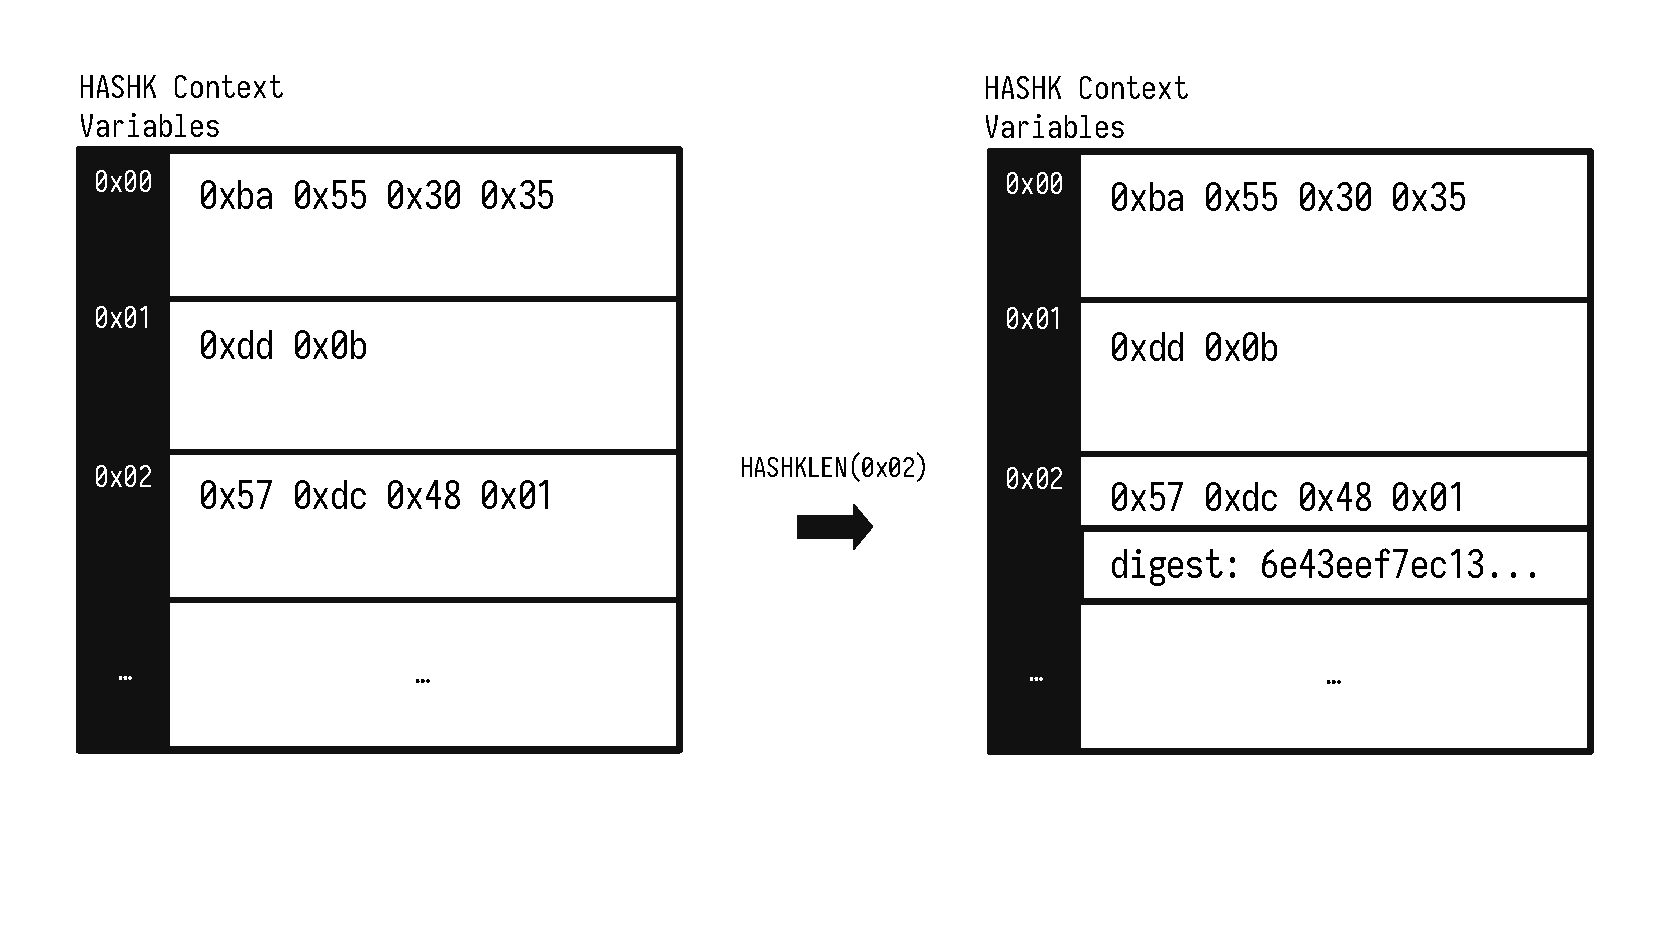
\includegraphics[width=0.6\columnwidth]{\assemblydir/figures/hashklen}
    \caption{Schema of the \HASHKLEN instruction.}
    \label{fig:hashklen}
\end{figure}


Following the previous example, the line of zkASM that we need to execute in this step is the following one:

\begin{zkasm}
    HASHPOS	:HASHKLEN(E)
\end{zkasm}

Recall that \texttt{HASHPOS} value at the current state is $32$ because we want to hash a total amount of $32$ bytes. 


More specifically, if $(h_1, \dots, h_k)$ is the input array attached to a specific address $\texttt{addr}$ (that is, $\mathtt{hashk}[\texttt{addr}] = (h_1, \dots, h_k)$ with the previous notation), the instruction

\begin{zkasm}
    len		:HASHKLEN(addr)
\end{zkasm}

internally stores the digest
\[
d = \texttt{KECCAK-256}(h_1, \dots, h_k).
\]

Observe that we should have that $k = \texttt{len}$. Otherwise, the \HASHKLEN instruction will get an error. % TODO: This checks are checking the integrity of the memory?




\subsubsection{\HASHKDIGEST}

This usual way we are invoking this instruction is the following 

\begin{zkasm}
    $ => REG	:HASHKDIGEST(E)
\end{zkasm}

Meaning that we are storing the digest of the hash attached to the address $\E$ into the register \texttt{REG}. The hash digest is introduced as a free input using the \texttt{\$ =>} operator. In our example, if we want to assign the digest of the hash to the register \D, we would use the following line

\begin{zkasm}
    $ => D		:HASHKDIGEST(E)
\end{zkasm}


%TODO: Counters needs to be incremented.



